%%!TEX root = diss.tex

\chapter{Collisional model of sediment velocity distributions}
\label{ch:langevin}
\section{Introduction}

Bulk bed load transport rates show wide and frequent fluctuations which originate from coupling between the fluid and granular phases.
Due to these fluctuations, measured transport rates often show extremely slow convergence through time, and predicted rates often deviate from measured values by several orders of magnitude.
These challenges limit numerous ecological and engineering applications that rely on sediment transport predictions.
In recent decades, stochastic formulations of the bed load flux have become increasingly popular for their potential to predict the mean transport rates required by applications while also predicting fluctuations, quantifying the dependence of measurements on the observation scale, and linking bulk transport characteristics to the ``microscopic" dynamics of individual grains.
Recent indications that sediment transport fluctuations might explain longstanding and unsolved problems in alluvial channel stability, such as channel width maintenance \citep{Boltzman, Lajeunesse2020} and bedform initiation \citep{Ancey2014,Bohorquez2016} provide additional motivation to develop these stochastic approaches.
One subset of these methods expresses downstream transport rates as a sum over the instantaneous streamwise velocities of all particles in motion within a control volume.
These approaches highlight the instantaneous velocity distribution of sediment particles as an object of crucial importance.
Unfortunately, current understanding of bedload velocity distributions remains limited.
We have as of yet no consensus on the shape of the bedload velocity distribution (is it Exponential, Gaussian, Gamma, or some other shape?), and no mechanistic models have yet been developed to describe the full range of experimental observations.
Here, we develop a stochastic model of particle velocities to addresses these issues.

Particle trajectories are a compromise between turbulent drag and particle-bed collision \citep{Wiberg1985}. We therefore anticipate that the Stokes number, which is known to characterize colliding bodies within a viscous fluid \citep{}, is an important dimensionless parameter of the bedload velocity distribution.
The Stokes number is defined as ... where ....

High-speed video experiments have measured different streamwise particle velocity distributions without providing much understanding as to why one distribution or another appears in a given set of hydraulic and sedimentary conditions.One set of studies has shown exponential particle velocity distributions \citep{Charru2004,Lajeunesse2010,Roseberry2012,Seizilles2014,Fathel2015,Fathel2016}.
These experiments involve uniformly-sized small sands or glass beads ($~0.05-2$mm) having typical Stokes numbers $St \sim 1-10$. Their flow conditions are generally sub-critical ($Fr<1$) and turbulent ($Re>5000$) but not always: flows in \citet{Lajeunesse2010} were super-critical ($Fr>1$), and flows in \citet{Charru2004} and \citet{Sezilles2014} were viscous.
A second set of studies have shown Gaussian particle velocity distributions \citep{Ancey2014,Heyman2016,Martin2012}. In these experiments, particles are typically larger ($2-8$mm) uniformly-sized gravels or glass beads having higher Stokes numbers ($St \sim 10-500$). In all Gaussian cases, flows are turbulent ($Re>5000$) and super-critical ($Fr>1$).
Two other experiments display velocity distributions that are intermediate between exponential and Gaussian and appear more like a Gamma distribution \citep{Houssais2012, Liu2019}. The \citet{Houssais2012} experiments involved a binomal distribution of glass beads with diameters $0.7$mm and $2.2$mm in turbulent and supercritical flow conditions. They resolved the velocity distributions for larger grains only. The \citet{Liu2019} experiments used uniformly-graded sand having median diameter $1.1$mm. Flows were again turbulent and subcritical.
From this experimental record, we can summarize that the shape of the velocity distribution does not consistentely relate to whether a flow is super or sub-critical ($Fr$), whether sediment grains are natural (sand, gravel) or synthetic (beads), or whether the flow is laminar or turbulent ($Re$). However, the typical Stokes numbers of particles do seem to increase monotonically from exponential velocity experiments (where $St \sim 1$), to intermediate (Gamma-like) experiments (where $St \sim 10$), and eventually to Gaussian experiments (where $St \sim 10^2$.) Apparently, the shape of streamwise bed load velocity distributions depends on the particle size.

Existing models of streamwise bed load velocities can be divided into computational and statistical physics categories.
Computational models numerically integrate some approximate coupled dynamics for individual grains and the fluid, generally modelling particles as spheres interacting through repulsive forces, and the flow using direct simulation of the Navier-Stokes equations or some related approximation (such as large eddy simulation or the St-Venant equations). When streamwise particle velocities have been analyzed in such simulations, they show exponential tails \citep{Gonzalez2017,Furbish2013} that agree with only a subset of the experimental data.
Statistical physics models have incorporated stochastic driving and resisting terms into the Newtonian dynamics of individual grains to develop a Langevin-like description of bed load particle motions.
For the downstream velocity $u(t)$, \citet{Fan2014} wrote $\dot{u} = F -\gamma \text{sgn}{u} + \xi(t)$ where $F$ represents the steady component of the fluid forcing, the term involving $\gamma$ is a quasi-static (Coulomb-type) friction term representing momentum dissipation by particle-bed collisions, and $\xi(t)$ is a Gaussian white noise representing variability in these forces. This model provides exponential velocity distributions which agree with one subset of experiments. \citet{Ancey2014} took a similar approach that includes different forces, solving $\dot{u} = \gamma(\overline{u}-u) + \xi(t)$. Here the term involving $\gamma$ is similar to a Stokes drag, except it involves the mean sediment velocity $\overline{u}$, not the fluid velocity as for a ``real" Stokes drag. $\xi(t)$ is again a Gaussian white noise representing fluctuations, and the model provides Gaussian velocity distributions that agree with another subset of experiments. 
While these models build insight into grain-scale sediment transport mechanics and provide powerful techniques with which to approach the problem, they have not yet provided a comprehensive explanation for the range of streamwise velocity distributions resolved in experiments.

Here, motivated by the realization that experimental particle velocity distributions vary systematically with the grain size, as summarized above, we hypothesize that the shape of the streamwise velocity distribution is controlled by the momentum dissipation characteristics of particle-bed collisions.
It is well-known that the elasticity of granular collisions within viscous fluids depends on the particle size.
In addition, the velocity distributions of granular gases are known to develop increasingly heavier tails than the Gaussian (Boltzmann) form of elastic gases as the inelastiscity of particle-particle collisions is increased.
Taking inspiration from this established knowledge, we develop below a model for sediment grains in transport as they undergo inelastic particle-bed collisions. Our intentions are to test the hypothesis that particle-bed collision characteristics explain the range of experimentally-observed streamwise bed load particle velocity distributions, and to introduce more realistic forces into earlier statistical physics descriptions of individual bed load particle dynamics. 
We develop the model and explain our assumptions in section \ref{sec:model}, then we present the analytical solution and major results in \ref{sec:results}. We finally discuss the implications of these results, summarize our findings, and suggest ideas for further research in sections \ref{sec:discussion} and \ref{sec:conclusion}.


\section{Model}
\label{sec:model}

Figure \ref{fig:1} indicates the configuration we have in mind. Nearly spherical and cohesionless particles of diameter $d$ and mass $m$ moving as bed load down a slope inclined at an angle $\theta$ in a steady turbulent shear flow. The flow is just strong enough to drive grains into rarefied transport of a kind typical in gravel-bed rivers: particles saltate along the bed in sequences of collisions between events of erosion and deposition; moving particles collide often with stationary particles, but rarely with other moving particles.
Particles respond to turbulent drag forces $F_D(t)$ and episodic particle-bed collision forces. In contrast to the computational physics approach, we do not aim to characterize the exact timeseries of the forces on an individual particle. Instead, we model the ensemble of possible force timeseries that particles could conceivably experience. Each possibility implies a different velocity timeseries $u(t)$ in the downstream direction.
Our objective is to calculate the probability distribution $P(u)$ of this downstream velocity by averaging over the ensemble of forces.
We include the most realistic article-bed collision and fluid forces we can while still allowing for analytical solutions. 

Collision forces dissipate streamwise momentum, partly by converting it to vertical, lateral, or rotational momentum, and partly by deforming particles and generating heat \citep{Williams2020}.
The microscopic details of particle-particle collisions have been thoroughly studied \citep{Brach1989, Lorenz1997,Montaine2011}. Here, we introduce a restitution-like coefficient $\varepsilon$ as indicated in figure \ref{fig:1}. This ranges from $\varepsilon=0$ for completely inelastic collisions to $\varepsilon=1$ for completely elastic collisions.
If the streamwise velocity just prior to a collision is $u$, just after the collision it becomes $\varepsilon u$. 
\begin{figure}
	\centerline{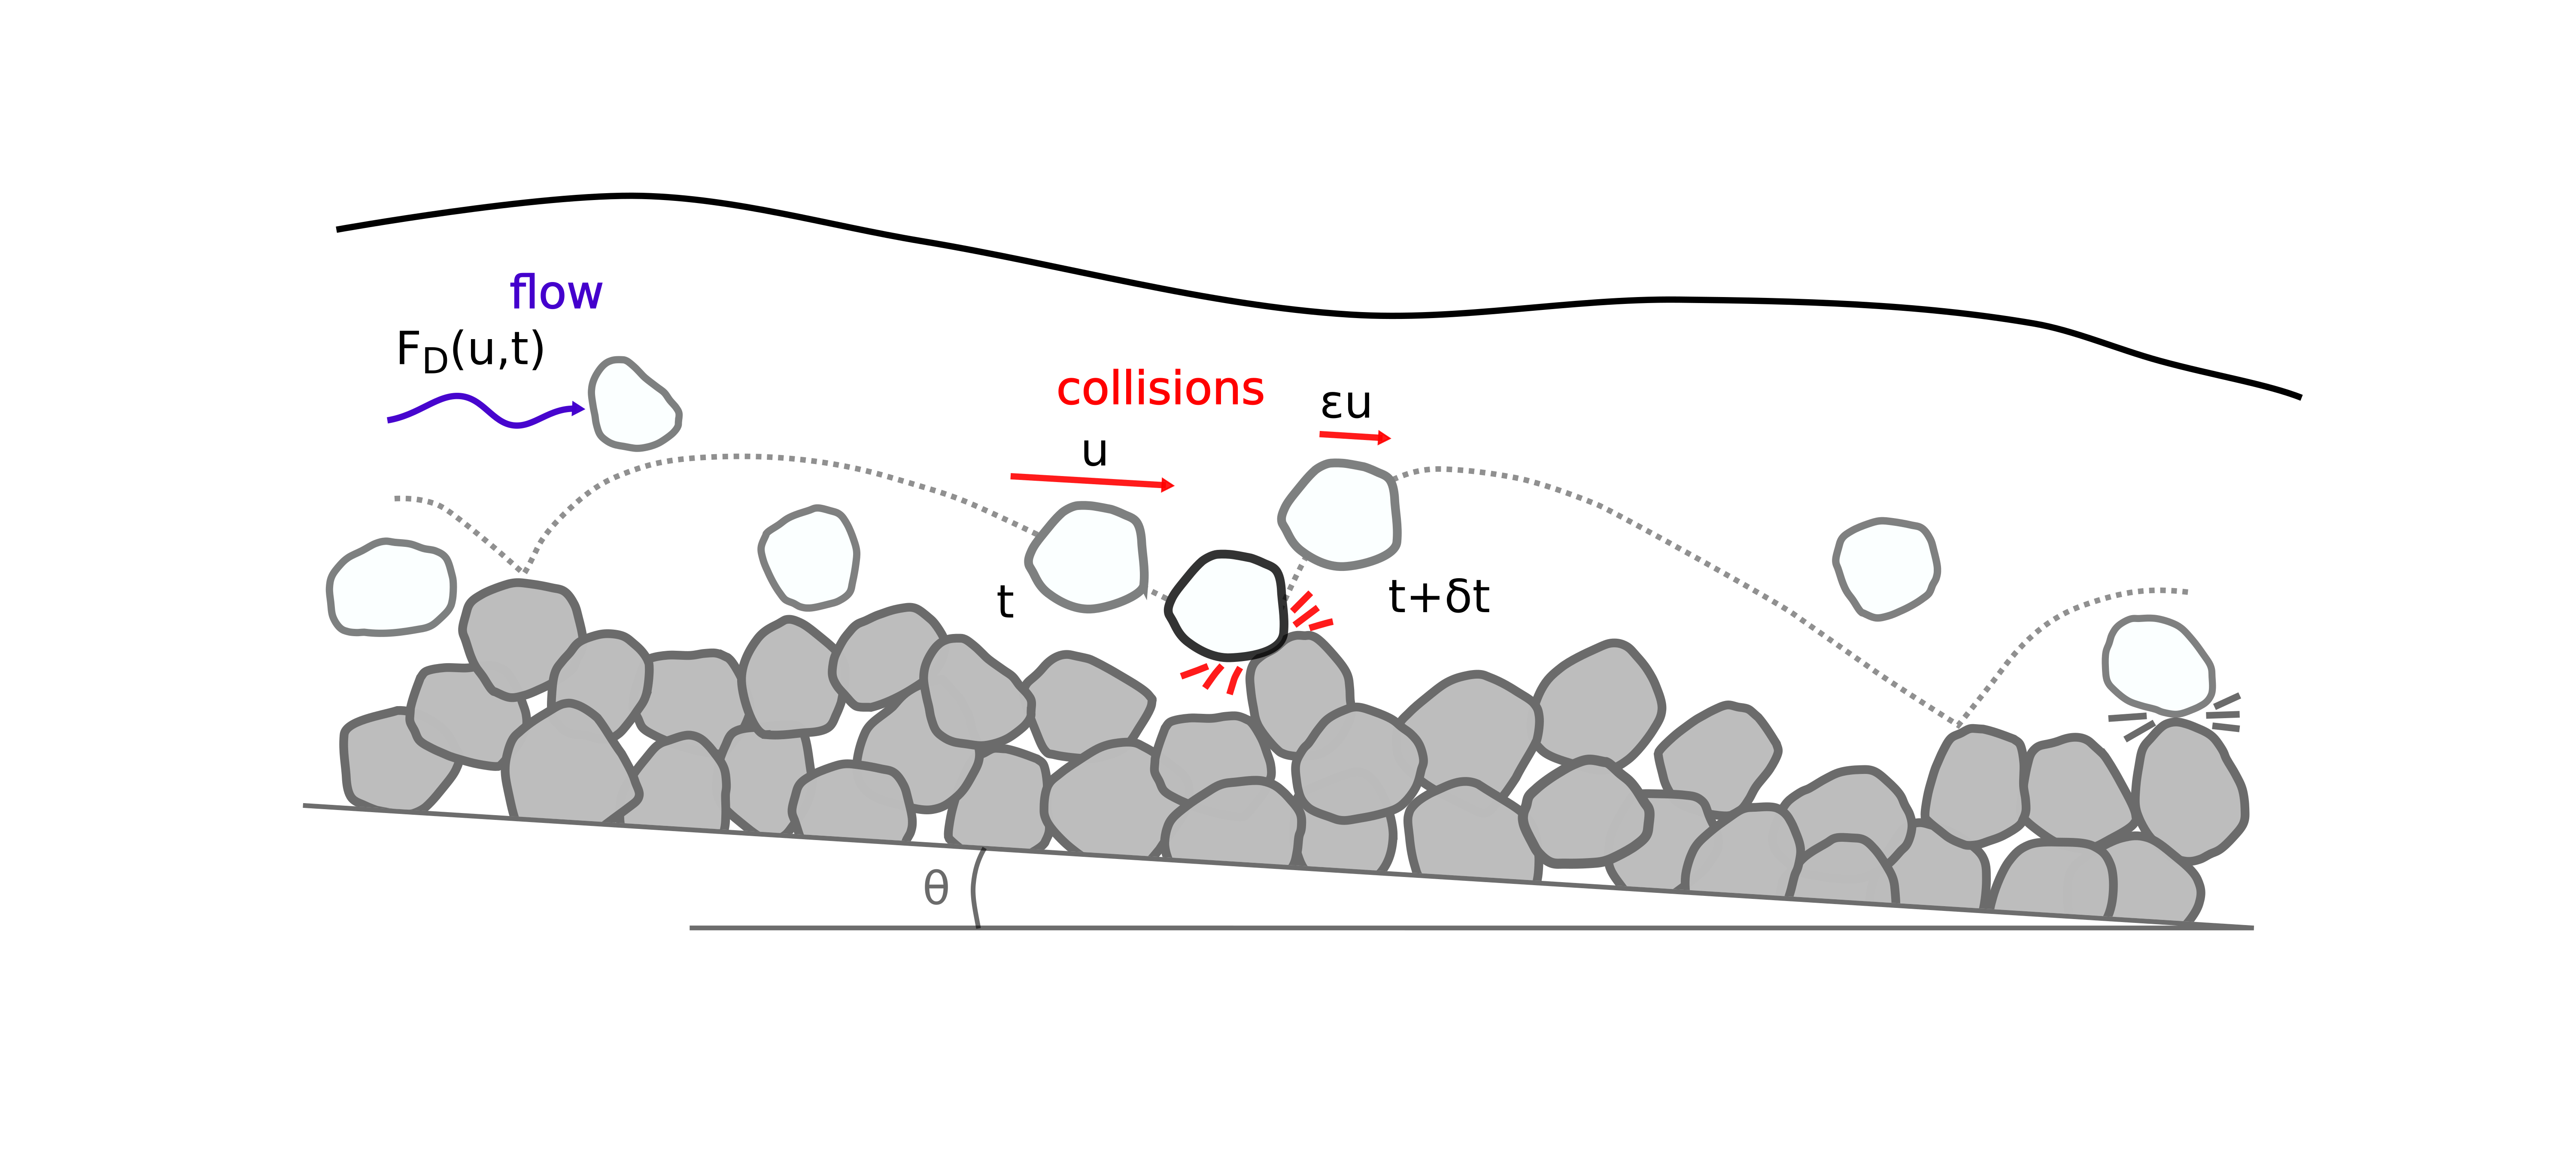
\includegraphics{./figures/ch5/Fig1Concept.png}}
	\caption{Definition sketch of rarefied sediment transport with turbulent fluid drag and particle-bed collision forces. During saltation, pre-collisional streamwise velocities $u$ are transformed to postcollisional velocities $\ve u < u$.}
	\label{fig:fig1}
\end{figure}
Since this quantity combines effects of particle shape and collision geometry and should vary from one collision to the next, we consider that the fraction of streamwise momentum dissipated per collision $\varepsilon$ lies on a statistical distribution $\rho(\varepsilon)$.
Similar ideas are available in the granular physics literature \citep{Serrero2015}.
Further assuming that the number of collisions per unit time is $\nu$ and that the time intervals between subsequent particle-bed collisions are exponentially distributed \citep{Gordon1972}, we write the collision force in the downstream direction as
\be F_C(u,t) = - m u \sum_{k=1}^{N_\nu(t)}(1-\varepsilon_k)\delta(t-\tau_k). \label{eq:col} \ee
Here, $N_\nu(t)$ is the number of collisions in time $t$, the $\tau_k$ ($k=1,2,\dots$) are times at which collisions occur, and the $\varepsilon_k$ are elasticity coefficients characterizing the amount by which each collision slows the particle down.
This collision force is a sequence of random impulses which are proportional to the pre-collisional streamwise momentum. This collision model should be adequate when the contact times between moving and resting particles are small compared to the times between collisions. These conditions are always satisfied for the idealized saltation-type motion depicted in figure \ref{eq:1}.

Fluid forces on a coarse particle in a viscous flow depend on the Reynolds number $\Rey_p = d V/\nu$ defined by the particle size $d$, slip velocity $V$ between particle and fluid, and kinematic viscosity $\nu$.
These forces have been calculated analytically from the Navier-Stokes equations for vanishing $\Rey_p$ and include acceleration, history, and velocity-dependent drag terms \citep{Hjelmfelt1966, Maxey1983, Auton1987}.
At realistic $\Re_p$ analytical results are limited, so it is standard practice to turn instead to empirical corrections on the small $\Rey_p$ formulas \citep{Schmeeckle2007,Mei2006}.
A dominant contribution to the downstream drag force $F_D$ on nearly spherical particles at large $\Re_p$ can be written $F_D = \frac{\pi}{8}
\rho_f d^2 C_D(\Rey_p) |V|V$, where $\rho_f$ is the fluid density, $d$ is the particle diameter, $C_D(\Rey_p)$ is an empirical drag coefficient, and $V = U-u$ is the slip velocity between the fluid ($U$) and particle ($u$) velocities \citep{Coleman1967, Schmeeckle2007, Dwivedi2012}.
In the present model we set $C_D = \frac{24}{\Rey_p}( 1 + 0.194 \Rey_p^{0.631})$ \citep{Clift1978,Gonzalez2017} and we do not involve acceleration and history terms for simplicity, although we acknowledge their potential importance for coarse sediment transport \citep{Michaelides1995,Armenio2001,Dalche2015}.

Drag forces have been argued to fluctuate rapidly compared to the inertial response times of coarse sediment grains \citep{Fan2014}.
The magnitude of drag fluctuations has been observed to follow a Gaussian distribution \citep{Hofland2006,Schmeeckle2007,Dwivedi2010,Celik2014}.
Using these ideas, we make two key simplifications of the drag force above.
First, we split the drag $F_D$ into quasi-steady and fluctuating components \citep{Michaelides1997}, and second, we represent drag fluctuations as a Gaussian white noise characterized by a particle diffusivity $D$ \citep{Fan2014,Ancey2014}. 
Defining $\bar{V}$ as a representative slip velocity which we specify more carefully later,  $\bar{C}_D$ as the empirical drag coefficient evaluated at this slip velocity, and $\xi(t)$ as a Gaussian white noise of mean $0$ and variance $1$ \citep{Gardiner1983}, we express the fluid forces as
\be F_D(t) = \frac{\pi}{8}
\rho_f d^2 \bar{C}_D \bar{V}^2 + \sqrt{2 D } \eta(t). \ee
In this drag force \ref{eq:drag} and the collision force \ref{eq:col}, the turbulent fluctuations $\xi(t)$, collision times $\tau_k$, and dissipation coefficients $\varepsilon_k$, can take any values consistent with their distribution and correlation functions. This set of possiblities defines a statistical ensemble.

\subsection{Langevin equation}

With the above forces, we express the Langevin equation $m\dot{u}(t) = F_D(t) + F_C(t)$ for the sediment dynamics as
\be m \dot{u}(t) = \Gamma + \sqrt{2D}\eta(t) - m u(t) \xi_{\nu, \ve}(t). \label{eq:langevin} \ee
This equation replaces the steady friction terms of earlier stocahstic bed load models with an episodic term which provides a more realistic representation of particle-bed collisions during saltation.
It represents a jump-diffusion process \citep{Daly2006} with multiplicative Poisson noise \citep{Dubkov2016,Denisov2009}. 
Collisions introduce ``jumps" in velocity while turbulent generates "diffusion".
The collision term is "multiplicative" in the sense that $u$ multiplies the Poisson noise.
Equations like \ref{eq:langevin} have long been studied in the stochastic physics literature \citep{Hanggi1978,vandenBroek1983}, but solving such equations remains extremely challenging \citep{Luczka1995,Daly2010,Mau2014,Dubkov2019}.
One issue is that multiplicative white noises imply the prescription dilemma of stochastic calculus \citep{Risken1984,Gardiner1983}, meaning \ref{eq:langevin} is not defined without further specifying an integration rule \citep{Suweiss2011}.
Here, the Ito interpretation (lower endpoint integration rule) is the physical choice since the energy dissipated by collisions depends strictly on pre-collisional velocities, not post-collisional.
Given this integration rule, the remaining issues are to obtain the integro-differential equation characterizing the ensemble of velocities defined by \ref{eq:langevin}, and then to solve this equation for the velocity distribution $P(u)$.

\subsection{Chapman-Komogorov equation and particle-bed collision integral}

We derive the equation governing the streamwise velocity distribution $P(u,t)$ from a simple limiting argument in appendix \ref{sec:appendixA}, finding
\be \nu^{-1}\partial_t P(u,t) = - \tilde{\Gamma} \partial_u P(u,t) + \tilde{D} \partial_u^2 P(u,t) + \mathcal{I}_c(u,t). \label{eq:master} \ee
In this equation, we introduced the scaled parameters $\tilde{\Gamma} = \Gamma/(\nu m)$ and $\tilde{D} = D/(\nu m)$. The term
\be \mathcal{I}_c(u,t) = - P(u,t) + \int_0^1 \frac{d\ve}{\ve}P\big(\frac{u}{\ve},t \big) \rho(\ve) \label{eq:colint} \ee
is a ``collision integral" term representing particle-bed collisions.
Equation \ref{eq:master} is a nonlocal extension of the Fokker-Planck equation used in earlier bed load models \citep{Fan2014,Ancey2014}. 
Such equations combining are known as Chapman-Komogorov equations \citep{Gardiner1983}. 
Nonlocality is introduced by the collision integral \ref{eq:colint} which transfers probability from higher pre-collisional velocities $u/\varepsilon$ to lower post-collisional velocities $u$.
This term is analogous to the collision integral of the Boltzmann equation in kinetic theory and granular gases \citep{Duderstadt1971, Brilliantov2004}. Physically, it corresponds to binary collisions between particles having different masses and random resitution coefficients \cite{Serero2015} in the limit that the mass of one particle (here, the particle resting on the bed) goes to infinity. Mathematically, it represents the probability distribution of the product between $\varepsilon$ and $u$ \citep[c.f.][]{Feller1968}.

Owing to its nonlocality, equation \ref{eq:master} does not admit analytical solutions as is, so we make one further approximation.
We assume the distribution of dissipation coefficients $\rho(\varepsilon)$ is sharply peaked at some most common (mode) value $\varepsilon'$. This allows for a Kramers-Moyal type expansion of the particle-bed collision integral \citep{Gardiner1983}.
Expanding all terms in the integrand except $\rho(\varepsilon)$ provides
\be \mathcal{I}_c(u,t) = -P(u,t) + \frac{1}{\varepsilon'}P\big(\frac{u}{\ve'},t \big) + \sum_{k=1}^\infty \frac{\alpha_k }{k!}(\ve - \ve')^k \Big[\frac{1}{\ve}P\big(\frac{u}{\ve}\big)\Big]^{(k)}\Big|_{\ve=\ve'},\label{eq:expansion}\ee
where the $\alpha_k = \int_0^1 d\ve \rho(\ve) (\ve-\ve')^k $ are the central moments of $\ve$ around the mode elasticity $\ve'$ and the superscript $(k)$ denotes the $k$th derivative.
In what follows, we drop all but the first two terms to obtain the leading order contribution of particle-bed collisions to the velocity distribution. Higher orders could always be included later by perturbation theory. We solve the resulting approximate equation in steady-state, when $\partial P(u,t)/\partial t = 0$. Scaling the time in Equation \ref{eq:master}, we can see this solution will be a good approximation to the time-dependent problem when particle motions generally survive multiple collisions.

\section{Results}
\label{sec:results}

\subsection{Derivation of the velocity distribution}
\label{sec:solution}
Hereafter we drop the prime on the most common streamwise restitution coefficient $\ve'$. With the truncation to two terms, equation \ref{eq:master} gives 
\be 0 = -\tilde{\Gamma}\partial_u P(u) + \tilde{D}\partial_u^2 P(u) -P(u) + \frac{1}{\ve} P\big(\frac{u}{\ve}\big),\label{eq:governer} \ee
which is now a non-local ordinary differential equation. Such equations have seen some attention in the mathematics literature, where they are called pantograph equations \citep{Hall1970,Zaidi2015,Bhalekar2017} for their relationship to a current collection device used on electric trains \citep{Ockendon1971}.
In the appendix we solve equation \ref{eq:governer} using Laplace transforms, providing
\begin{multline} P(u) = \frac{\theta(-u)}{K_+}\sum_{l=0}^\infty \frac{\ve^{-l}e^{\lambda_+\ve^{-l}u}}{\prod_{m=1}^l(-\tilde{D} \lambda_+^2 \ve^{-2m} + \tilde{\Gamma} \lambda_+ \ve^{-m} + 1) } 
	\\+ \frac{\theta(u)}{K_-}\sum_{l=0}^\infty \frac{\ve^{-l}e^{\lambda_-\ve^{-l}u}}{\prod_{m=1}^l(-d \lambda_-^2 \ve^{-2m} + \gamma \lambda_- \ve^{-m} + 1) } \label{eq:steadystate}. \end{multline}
The factors $\lambda_\pm$ are defined in the appendix; they are proportional to $\tilde{\Gamma}/\tilde{D}$. 
The normalization factors are $K_\pm$ are 
\be K_\pm = d(\lambda_+-\lambda_-)\prod_{l=1}^\infty (-d\lambda_\pm^2 \ve^{2l} + \gamma \lambda_\pm \ve^{l} + 1). \ee
Although this velocity distribution appears quite complicated, one can verify that this is a normalized probability distribution which has very simple limiting behaviors as the most common dissipation coefficient $\ve$ approaches fully elastic ($\ve=1$) and inelastic ($\ve = 0$) values.

It is rather simple to derive the moments of this probability distribution by multiplying \ref{eq:governer} by $u$, integrating, and then solving the resulting moment evolution equations \citep[c.f.][]{Cox1965}.
The first moment is
\be \langle u \rangle = \frac{\Gamma}{\nu(1-\ve)} = \frac{\gamma}{1-\ve},\ee
which is scales weakly with the mean fluid drag and sharply with the rate and typical elasticity of collisions.
The second moment is
\be \langle u^2 \rangle = 2 \frac{d + \gamma \langle u \rangle}{1-\ve^2}, \ee
leading to the velocity variance ($\sigma_u^2 = \bra u^2 \ket - \bra u \ket ^2 $)
\be \sigma_u = \sqrt{\frac{2 d + \gamma^2}{1-\ve^2}}.\ee
This equation demonstrates that velocity fluctuations originate from both the steady and fluctuating components of the flow forces, yet the variance is linear in these factors and is therefore relatively insensitive to them. In contrast, velocity fluctuations depend sharply on the parameters representing particle-bed collisions.

Figure \ref{fig:fig2} depicts velocity characteristics for different realizations of the fluid and collisional forces.
\begin{figure}
	\centerline{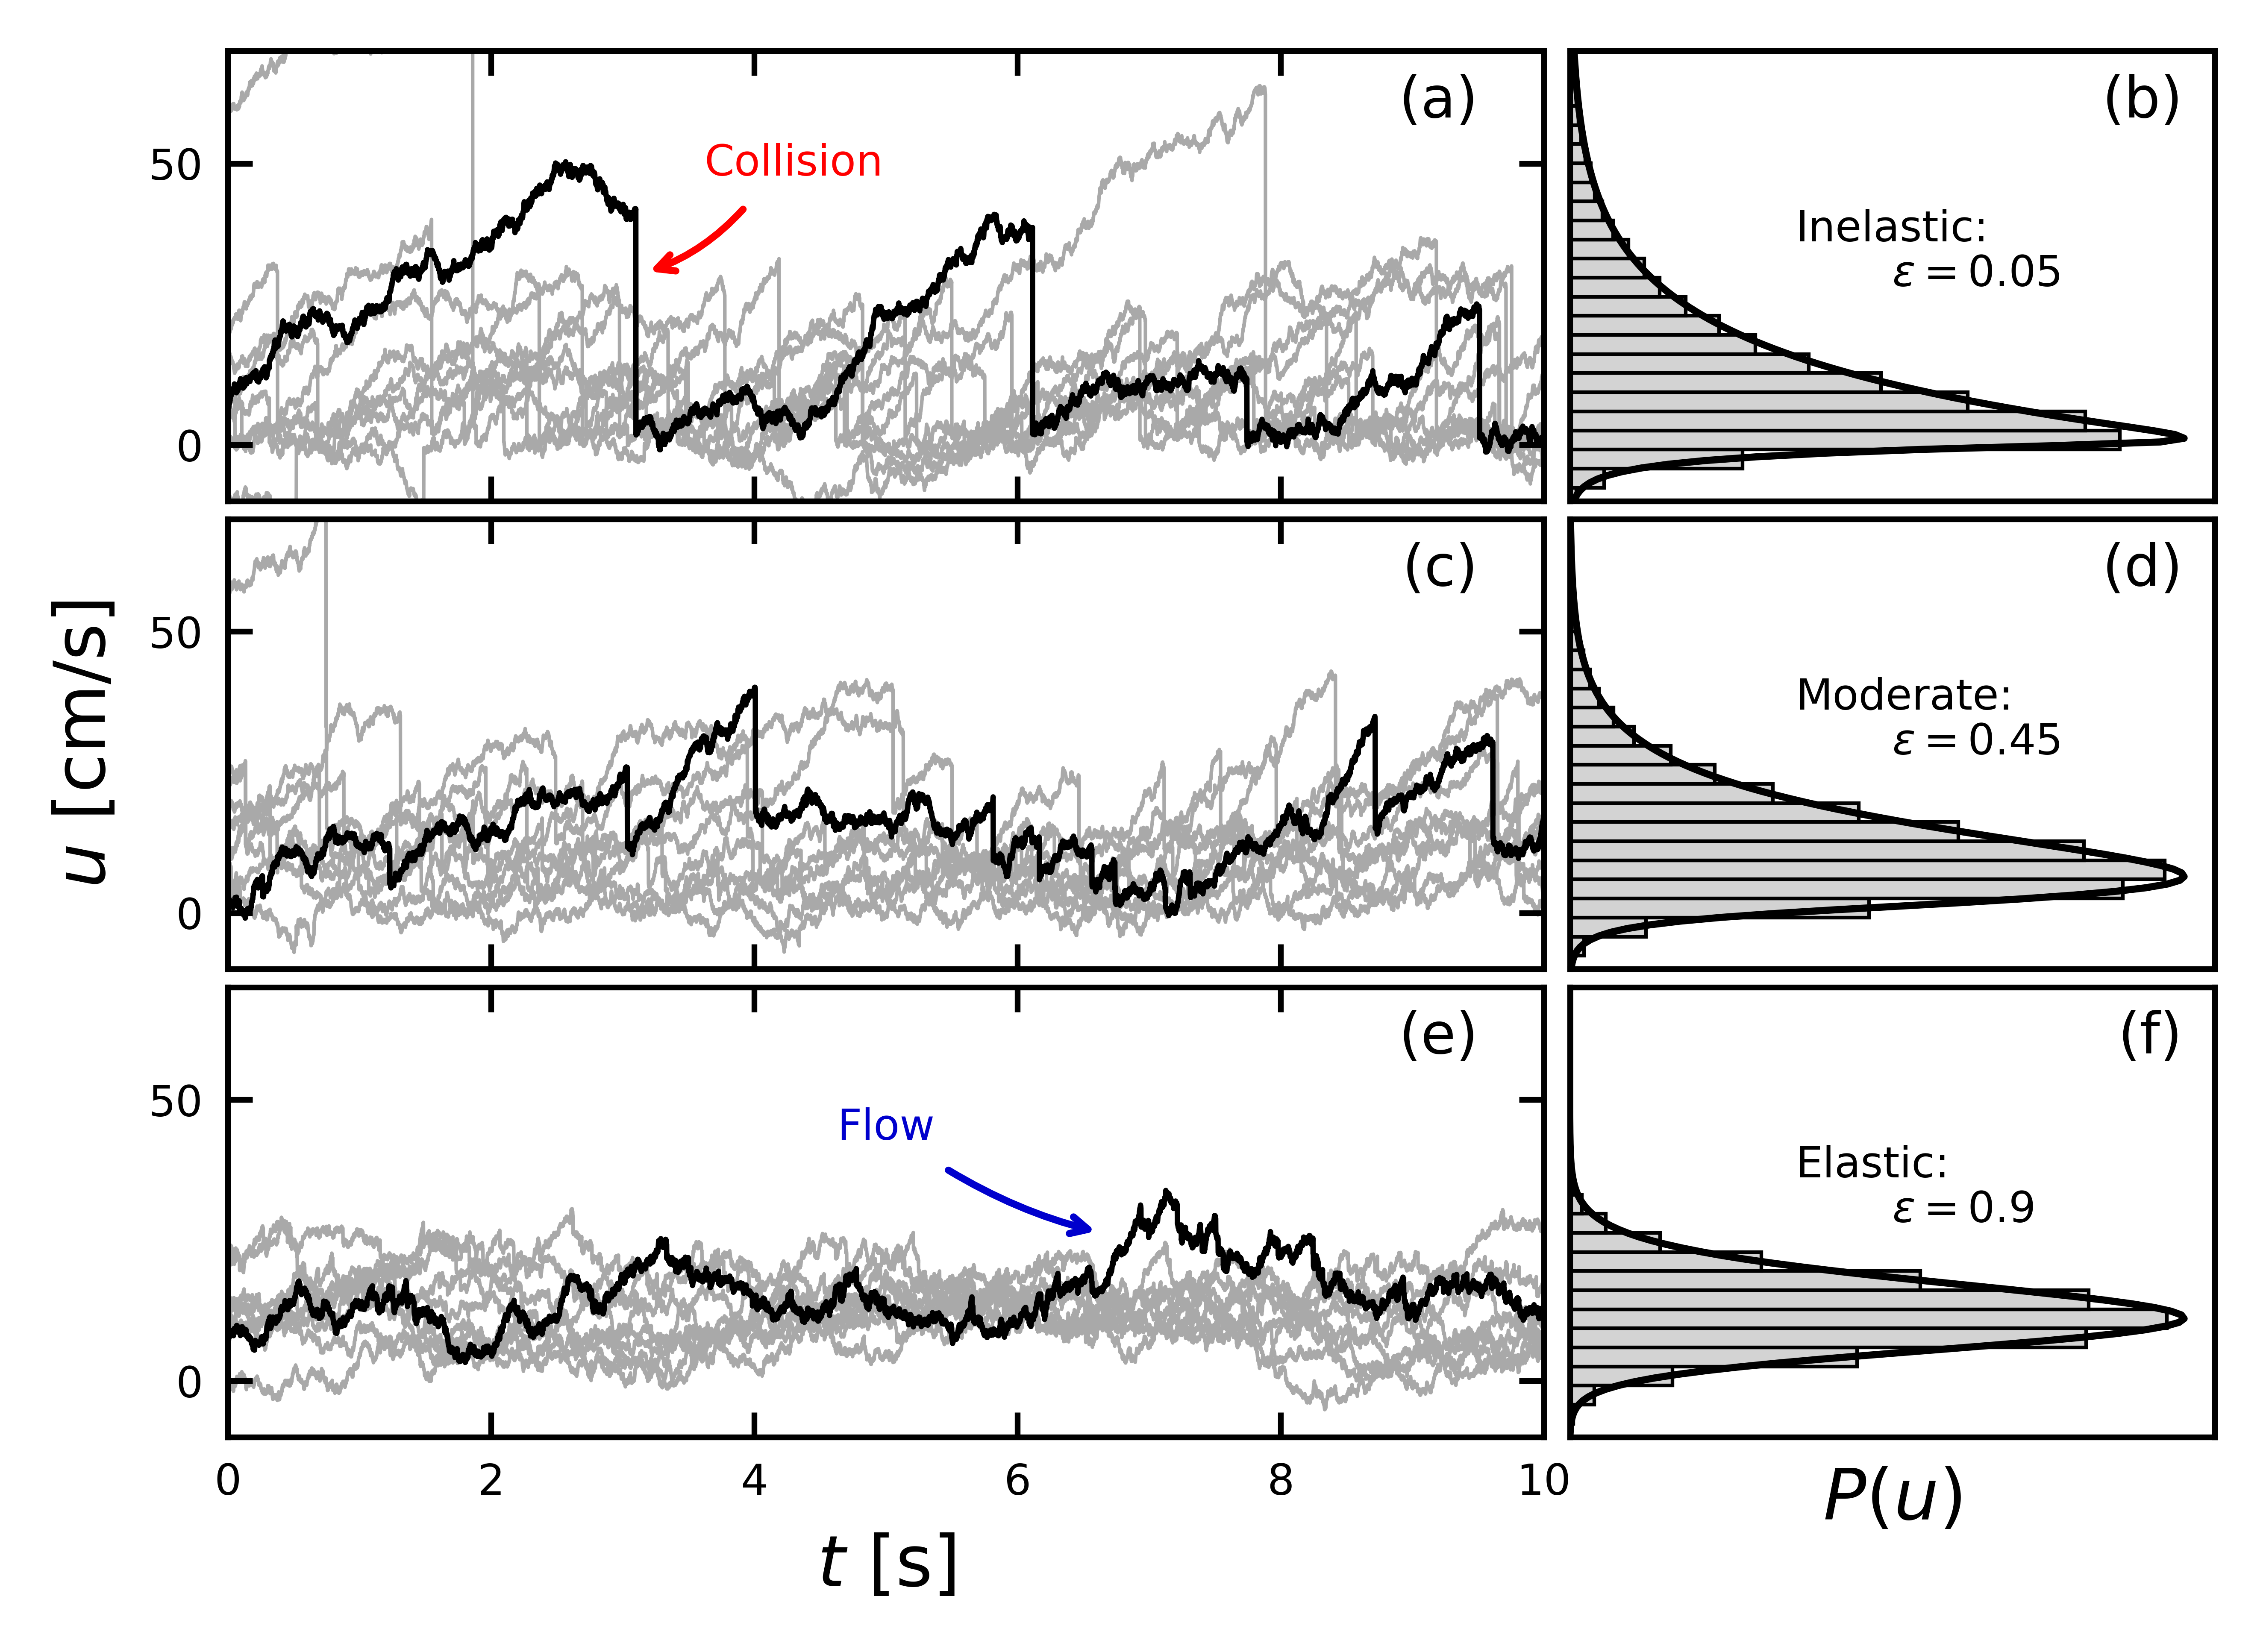
\includegraphics{./figures/ch5/Fig2pdfs.png}}
	\caption{Left panels show velocity realizations as gray traces. Velocities are calculated from Monte Carlo simulations. Individual realizations are singled out as black traces. Particle-bed collisions imply sudden downward-velocity jumps. Flow forces generate fluctuating positive accelerations between collisions. Right panels show simulated histograms of particle velocities and exact solutions from equation \ref{eq:steadystate}.}
	\label{fig:fig2}
\end{figure}
We can see an apparent transition from exponential-like to Gaussian-like velocity distributions as typical collisions vary from more inelastic ($\ve \rightarrow 0$) to more elastic ($\ve \rightarrow 1$). In between, the full distribution \ref{eq:steadystate} resembles a Gamma distribution, although it is not a Gamma distribution.


\subsection{Exponential and Gaussian regimes}
\label{sec:modelcomparison}

In fact, the apparent transition in figure \ref{fig:fig2} can be made rigorous: despite its complex appearance, simple Gaussian and exponential distributions appear as rigorous mathematical limits of equation \ref{eq:steadystate}. When particle-bed collisions are completely inelastic, \ref{eq:steadystate} becomes an exponential distribution, and when they are completely elastic, \ref{eq:steadystate} becomes Gaussian. Figure \ref{fig:fig3} demonstrates more closely the approach of the distribution toward these limits.
\begin{figure}
	\centerline{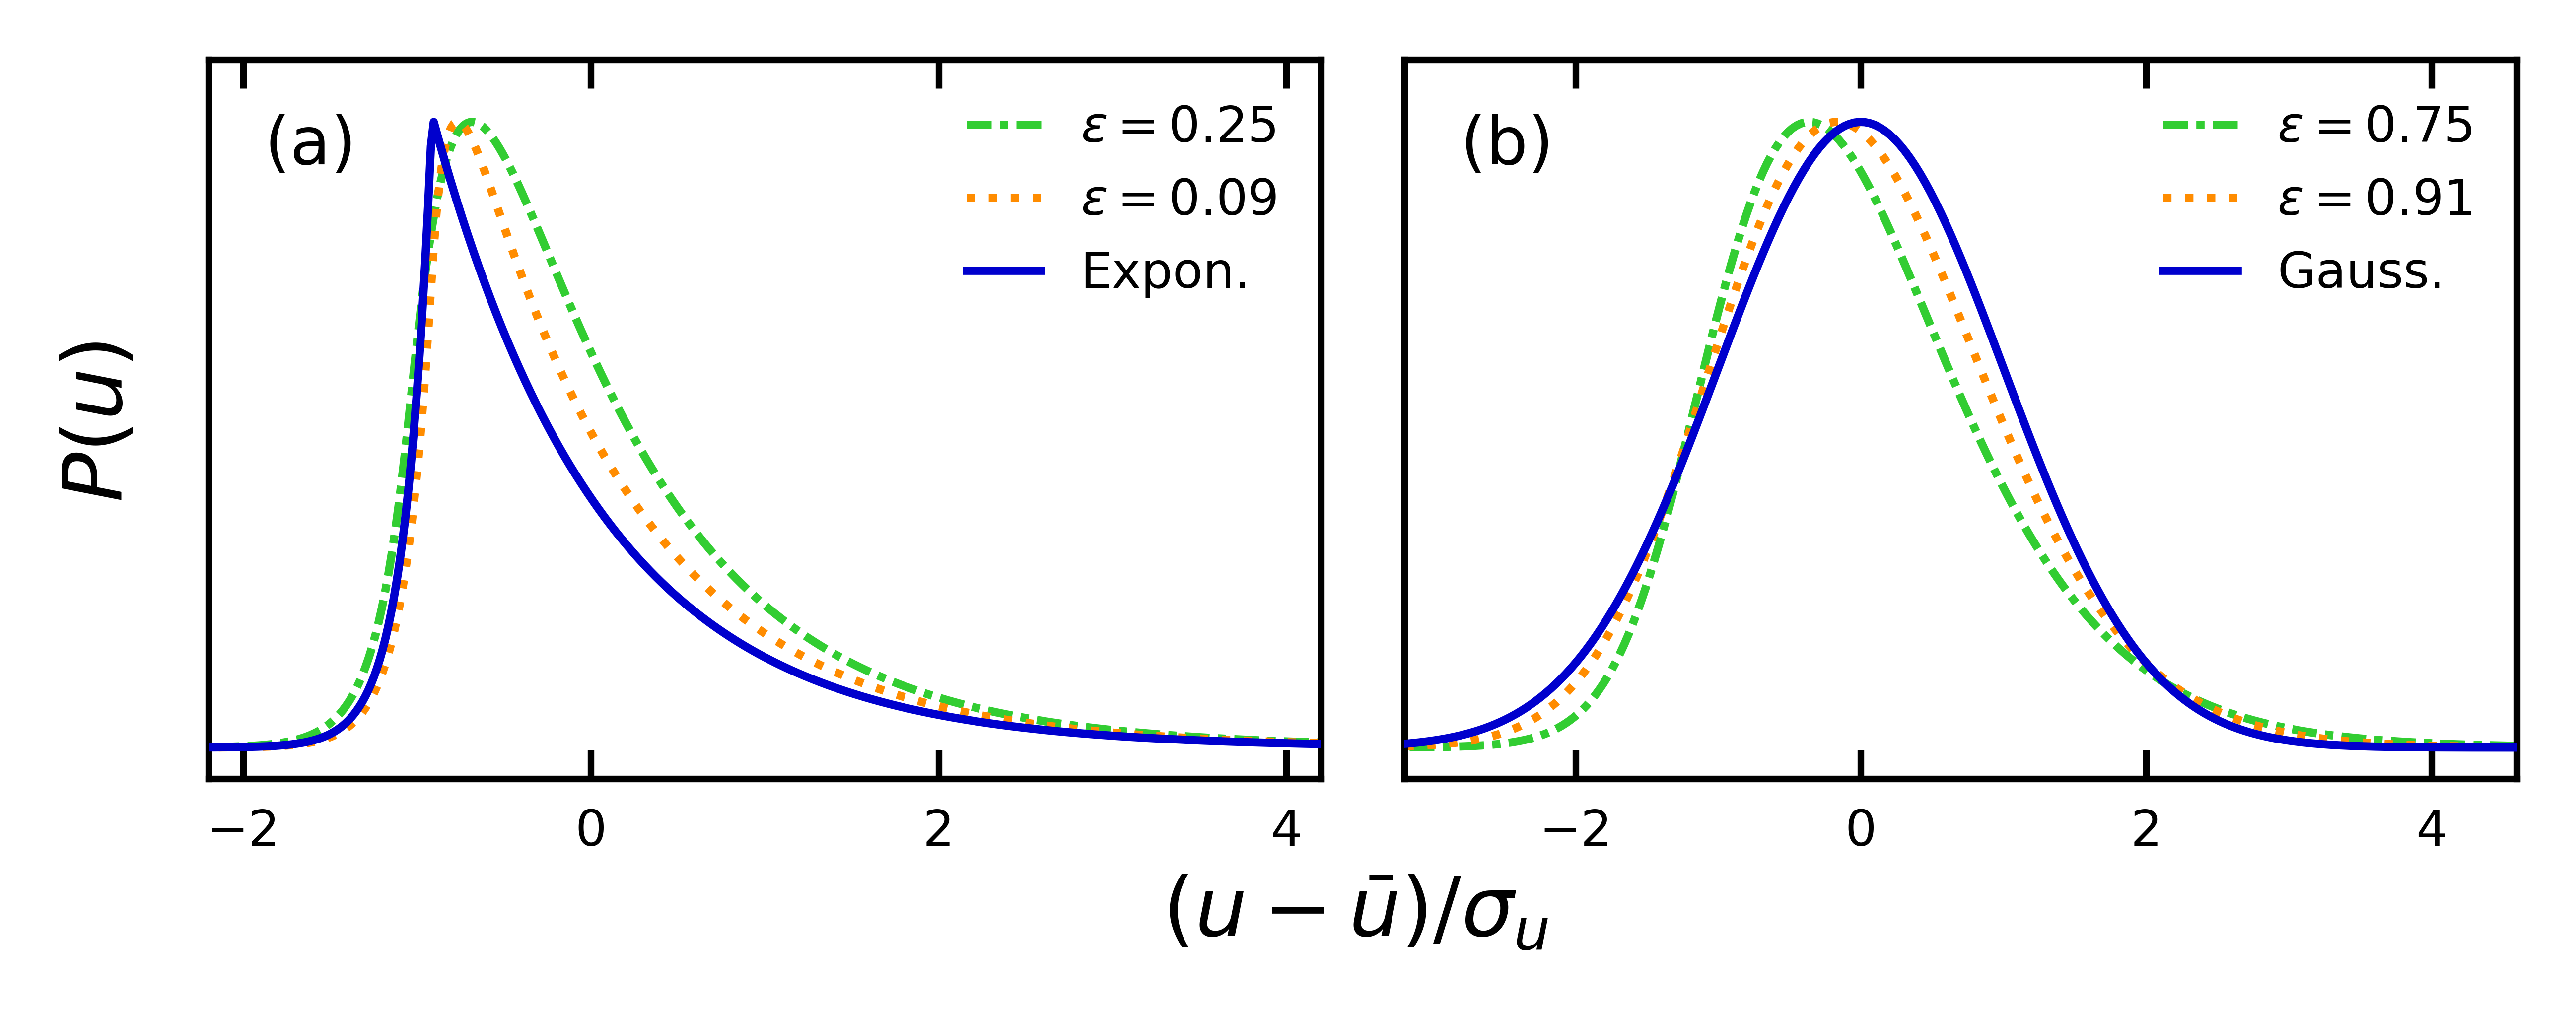
\includegraphics{./figures/ch5/Fig3asymptotic.png}}
	\caption{The particle velocity distribution approaches an exponential distribution in (a) as particle-bed collisions become extremely elastic ($\ve \rightarrow 1$), and it approaches a Gaussian in (b) as they become extremely inelastic ($\ve \rightarrow 0$). On the abscissa, the mean sediment velocity is standardized by its mean $\bar{u}$ and standard deviation $\sigma_u$. }
	\label{fig:fig3}
\end{figure}

The exponential limit of \ref{eq:steadystate} as $\ve \rightarrow 0$ is rather easy to see. Taking $\ve \rightarrow 0 $ in \ref{eq:steadystate}, all terms in the series except for that with $l=0$ become exponentially small, leaving behind the same two-sided exponential distribution derived by \cite{Fan2014} up to notational differences:
\be P(u) = \frac{d}{\sqrt{\gamma^2 + 4d}}e^{\frac{\gamma u }{2 d} - \frac{\sqrt{\gamma^2 + 4 d}|u|}{2d}}. \ee
Thus, for bed load transport conditions with typically very inelastic particle-bed collisions, we can expect exponential-like velocities and large deviations from a Gaussian behavior.

The Gaussian limit as $\ve \rightarrow 1$ of \ref{eq:steadystate} is more difficult to evaluate. The challenge is that the statistical moments \ref{eq:mean} and \ref{eq:2ndmom} diverge at the same time as the denominator factors of the distribution \ref{eq:steadystate}. In appendix \ref{sec:appendixB} we return instead to the original equation \ref{eq:governer} to evaluate this elastic limit, obtaining
\be P(u) = \frac{1}{\sqrt{2\pi\sigma_u^2}}e^{-\frac{(u-\bar{u})^2}{2\sigma_u^2}}. \label{eq:gaussian}\ee
This result is identical to the velocity distribution derived by \citet{Ancey2014}, up to notation.

\subsection{Comparison with experimental data}
\label{sec:experimentcomparison}

Now we compare the analytical distribution \ref{eq:steadystate} with the available experimental data.
Upfront, we point out that the distribution above has free parameters and this is only a proof of concept that the velocity distribution is capable of fitting the available experimental data; it is not a proof that this is the underlying mechanism for these data blahblahblah that was a good writing day.


\begin{table}
	\begin{center}
		\def~{\hphantom{0}}
		\begin{tabular}{lccc}
			$a/d$  & $M=4$   &   $M=8$ & Callan  \\[3pt]
			0.1   & 1.56905 & ~~1.56~ & 1.56904\\
			0.3   & 1.50484 & ~~1.504 & 1.50484\\
			0.55  & 1.39128 & ~~1.391 & 1.39131\\
			0.7   & 1.32281 & ~10.322 & 1.32288\\
			0.913 & 1.34479 & 100.351 & 1.35185\\
		\end{tabular}
		\caption{Values of $kd$ at which trapped modes occur when $\rho(\theta)=a$.}
		\label{tab:kd}
	\end{center}
\end{table}


\begin{figure}
	\centerline{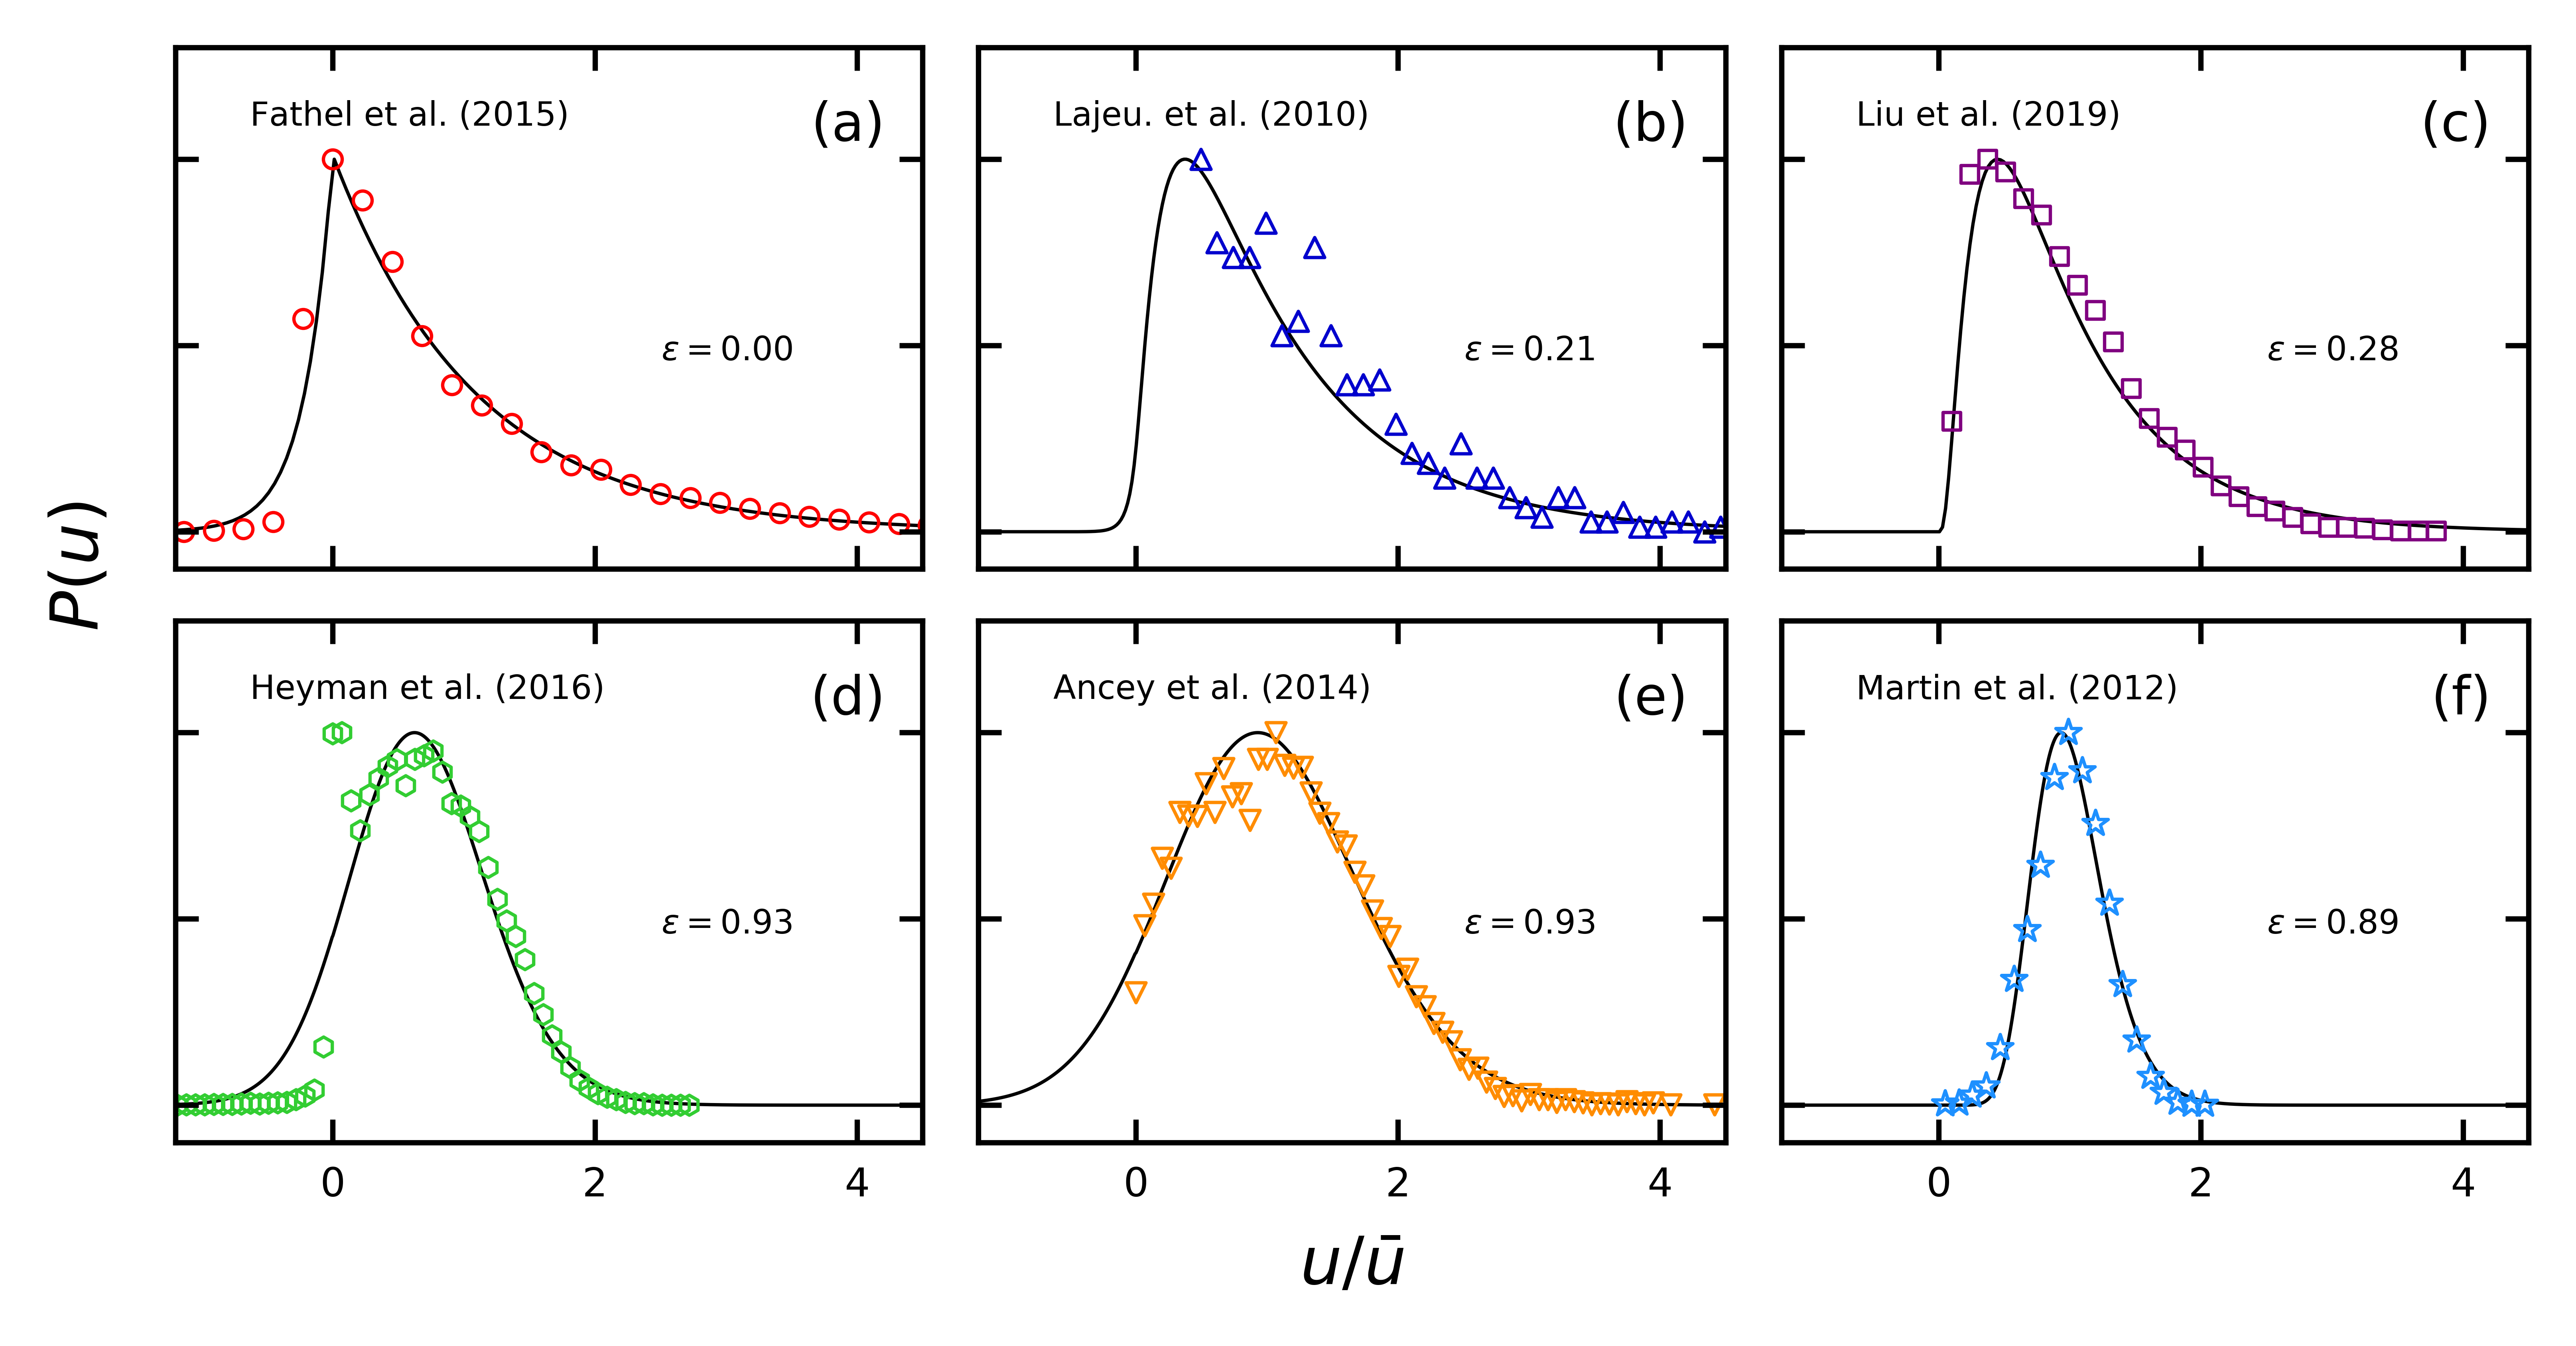
\includegraphics{./figures/ch5/Fig4expComparison.png}}
	\caption{The features of the four possible modes corresponding to
		(\textit{a}) periodic\protect\\ and (\textit{b}) half-periodic solutions.}
	\label{fig:fig4}
\end{figure}


\section{Discussion}
\label{sec:discussion}

Here, I developed a Langevin description of bed load sediment transport which includes episodic collisions between particles and the bed.
The model relates the shape of the instantaneous streamwise particle velocity distribution to the elasticity of particle-bed collisions,
generalizes earlier approaches available in the literature which did not treat episodic collisions \citep{Ancey2014,Fan2014}, and provides a new physical explanation for the different streamwise sediment velocity distributions resolved in experiments.
Although in reality, the turbulent forces on moving sediment particles vary in a complex spatio-temporal way, we have approximated the fluid forces on bed load particles as spatially uniform Gaussian white noise. Even though the non-Gaussian aspects of fluid turbulence certainly do impact sediment entrainment \citep{Coleman2019,Celik2014}, this flow model appears more or less justified since sediment transport experiments provide similar velocity distributions regardless of whether the flow is viscous or turbulent \citep{Lajeunesse2010, Charru2004}, and since particle relaxation times are typically long compared to the timescales of turbulent fluctuations \citep{Hofland2006,Schmeeckle2007,Nakagawa1981}.
We modelled particle-bed collision forces as a sequence of instantaneous impulses where the intervals between successive collisions were characterized as exponential random variables. The effect of each collision on the streamwise particle velocities was parameterized by a restitution-like coefficient.
Although such approximate descriptions of particle-particle collisions are common in the theory of granular gases, the setting here is somewhat different than grains in air. Because particles within a viscous flow in general interact at a distance, we should expect the collision model will become poor when the time between subsequent collisions becomes small. Therefore, although the model seems appropriate for saltation, it should be critically examined for ``reptation", when the times between subsequent particle-bed collisions are short. Of course, more realistic flow and collision forces could always be incorporated into Langevin equations for bed load transport, although these might require numerical methods for their solution. The theory of granular gases provides some indication of the types of more nuanced collision models which are possible \citep{Brilliantov2004,other..}.

Sediment transport experiments reveal correlations between particle size and the shape of the bed load velocity distribution.
Experiments with smaller particles tend to give exponential distributions, and those with larger particles give Gaussian distributions.
In fluid dynamics, the dissipation characteristics of particle-particle collisions in viscous flows are known to depend on the particle size and approach velocity through the Stokes number. 
In kinetic theory, it is known that gases of ideal elastic particles generate Gaussian (Boltzmann) velocity distributions, while gases of inelastic grains generate non-Gaussian distributions \citep{Chapman1970,Brilliantov2004}.
Taken together, these ideas suggest that we might relate the shape of the particle velocity distribution to particle size.
We can estimate typical Stokes numbers of colliding bed load particles in experiments as $...$, using with the flow shear velocity and mean streamwise sediment velocity to calculate $V$. Estimating in this way, transport experiments with exponential velocities have $St \sim 1-10$, those with neither exponential nor Gaussian velocities have $St \sim 10-100$, and those with Gaussian velocities have $St > 100$.
In experiments relating restitution coefficient to Stokes number for idealized collisions, restitution coefficients vary sharply from $0$ to $1$ as $St$ ranges from $1$ to $500$ \cite{Marshall2001,Joseph2001,Yang2006}.
Although collision geometry and grain shape certainly complicate the narrative, these values of $St$ are consistent with our model conclusion that the shape of the particle velocity depends on the elasticity of collisions.

In real channels, grain sizes often span a wide range. A major implication of the dependence of the shape of the particle velocity distribution on grain size is that different grain sizes in a mixture will impart distinct fluctuation signatures to the overall bulk transport rate. Even in the absence of sorting effects and differential mobility, smaller grains can be expected to carry more control over the largest fluctuations in the overall transport rate, since their velocity distributions have wider tails. 

\section{Implications for landscape evolution}

Many phenomena of landscape evolution depend on the velocities of individual grains.
The erosion rates of bedrock rivers are for example parameterized by the impact velocities of individual sediment grains against the bedrock surface \citep{Skylar2004,Tingian,Turowski2020}, on which they have a sensitive nonlinear dependence.
It is not much of a stretch to imagine that bedrock erosion could be dominated by the largest impact velocities that originate from the extreme tail of the bedload velocity distribution. Here, we have shown that the weight of this tail depends sensitively on the dissipation characteristics of particle-bed collisions, suggesting that another feedback, that between dissipation and ... may be at play in the evolution of bedrock canyons.

\section{Rivers, hillslopes, and dunes}

It has long been recognized, probably since \citet{Bagnold1941} and certainly today \citep{}, that there are deep analogies between tranpsort phenomena in air and water.
In an ideal perspective, we might imagine writing the governing equations for transport in water as a function of the fluid viscosity, then tuning the viscosity between air and water to obtain a description applying to both spheres.


For example, in a mixture of small and large grains, neglecting any sorting effects whereby the mobility of small grains is contingent on the mobility of the large grains, small grains will have exponential velocities with relatively wide fluctuations, while large grains will have Gaussian velocities with relatively narrow fluctuations. Considering the over-all flux then as the number of moving particles times their velocities, transport fluctuations



aeolean transport extension maybe
particle size distributions - interesting implications
connection to computational physics approach
connection to the stochastic description of the flux





\section{Conclusion}
We have demonstrated that particle-bed collisions control the shape of the particle velocity distribution.  
\label{sec:conclusion}


\appendix

\section{Derivation of Master Equation}
To derive the master equation from \ref{eq:langevin}, we temporarily consider the Gaussian white noise (GWN) $\xi(t)$ as a Poisson jump process having rate $r$ and jumps $ \sqrt{2 d} h$ with $h$ distributed as $f(h)$. We will later take a GWN limit on this noise. With this assumption, integrating \ref{eq:langevin} over a small time interval $\delta t$ considering the Ito interpretation for the collision term provides
\be     
u(t+\delta t) =
\begin{cases}
	u(t) + \gamma \delta t & \text{with probability } 1- r \delta t - \nu \delta t\\
	u(t) + \sqrt{2 d} h &  \text{with probability } r \delta t \\
	\ve u(t) &  \text{with probability } \nu \delta t
\end{cases}
\ee

Considering the probability $P(u,t+\delta)$ as sum over possible paths from $P(u,t)$ develops 
\begin{align} P(u,t+\delta t) =
	(1- r \delta t - \nu \delta t)\int_{-\infty}^\infty dw  \delta(u-w-\gamma \delta t) P(w,t)\\ 
	+  r \delta t \int_{-\infty}^\infty dw \int_{-\infty}^\infty dh f(h) \delta (u - w - \sqrt{2 d}h) P(w,t) \\ 
	+ \nu \delta t \int_{-\infty}^\infty dw \int_0^1 d\ve \rho(\ve)  \delta(u-w\ve) P(w,t).
\end{align}
Evaluating all integrals over $\delta$-functions provides 
\begin{align} P(u,t+\delta t) = (1-r \delta t - \nu \delta t)P(u-\gamma \delta t, t) \\+ r \delta t\int_{-\infty}^\infty dh f(h) P(u+\sqrt{2d}h) \\+ \nu \delta t \int_0^1 \frac{d\ve}{\ve} \rho(\ve) P\big(\frac{u}{\ve}\big).\end{align}
Finally, we take $\delta t \rightarrow 0$ and limit the Poisson noise involving $\sqrt{2d}$ to a Gaussian white noise by taking $r \rightarrow \infty$ as $h \rightarrow 0$ such that $h^2 r = 1$ \cite{VanKampen1983}. This process finally obtains the master equation (\ref{eq:master}).
\section{Derivation of Steady-state solution}

Defining $\tilde{P}(s) = \int_{-\infty}^\infty du e^{i u s} P(u) $ as the Fourier transform (FT) of $P(u)$ and taking the FT of \ref{eq:detlangevin} develops the recursion relation
\be \tilde{P}(s) = \frac{\tilde{P}(s\ve)}{q(s)}. \ee
where
\be q(z) = d z^2 - i \gamma z + 1 . \label{eq:q} \ee
Recursing $N+1$ times provides
\be \tilde{P}(s) = \frac{\tilde{P}(s \ve^{N+1})}{q(s \ve^0)q(s\ve^1)\dots q(s\ve^N)}.\label{eq:recursion}\ee
The polynomials $q(z)$ can always be factored as $q(z) = d(z - i\lambda_-)(z - i\lambda_+)$ where
\be \lambda_\pm = \frac{\gamma}{2d}\Big[1 \pm \sqrt{ 1 + 4d/\gamma^2} \Big].\ee
Using these factors to expand $\tilde{P}(s)$ in partial fractions provides
\be \tilde{P}(s)  = \tilde{P}(s \ve^{N+1}) \sum_{l=0}^N  \Big[ \frac{R_l^-}{s\ve^l - i\lambda_-} + \frac{R_l^+}{s\ve^l - i\lambda_+} \Big] \ee
where the coefficients $R_l^\pm$ are the residues of the product $[q(s\ve^0)\dots q(s\ve^N)]^{-1}$:
\be R_l^\pm = \frac{s \ve^{l} - i\lambda_\pm }{q(s\ve^0)\dots q(s \ve^N)} \Big|_{s= i \lambda_\pm \ve^{-l}}.\ee
The Fourier transform (\ref{eq:recursion}) has a beautiful feature as $N\rightarrow \infty$: since $0<\ve <1$, the prefactor $\tilde{P}( s \ve^{N+1})$ becomes the normalization condition $\tilde{P}(0)=1$ for the probability distribution $P(u)$ in the limit.
Taking this limit and evaluating the residues provides 
\begin{multline} \tilde{P}(s) = \frac{1}{d(\lambda_+ - \lambda_-) \prod_{m=1}^\infty q(i \lambda_- \ve^m)} \sum_{l=0}^\infty \frac{i}{(s\ve^l-i\lambda_-)\prod_{m=1}^l q(i\lambda_- \ve^{-m})} 
	\\+ \frac{1}{d(\lambda_+ - \lambda_-) \prod_{m=1}^\infty q(i \lambda_+ \ve^m)} \sum_{l=0}^\infty \frac{-i}{(s\ve^l-i \lambda_+)\prod_{m=1}^l q(i\lambda_+ \ve^{-m})} \end{multline}
Finally, inverting the Fourier transforms term by term with contour integration and incorporating (\ref{eq:q}) provides the steady-state solution (\ref{eq:steadystate}).

\section{Calculation of the moments}
Taking (\ref{eq:master}), multiplying by $u^k$, integrating over all space, and taking account of normalization of $P(u)$ provides a recursion relation for the moments: 
\be 0 = Dk (k-1)\langle u^{k-2} \rangle + \Gamma k \langle u^{k-1} \rangle + \nu (\ve^k-1)\langle u^k \rangle. \ee
$k=1$ provides the mean
\be \langle u \rangle = \frac{\Gamma}{\nu(1-\ve)} = \frac{\gamma}{1-\ve}\ee
while $k=2$ provides the second moment
\be \langle u^2 \rangle = 2 \frac{d + \gamma \langle u \rangle}{1-\ve^2}, \ee
leading to the velocity variance
\be \sigma_u = \sqrt{\frac{2 d + \gamma^2}{1-\ve^2}}.\ee
\section{Weak and strong collision limits}
Now we demonstrate that weak collisions imply a Gaussian-like distribution for sediment velocities. The limit is challenging since the steady-state distribution \ref{eq:steadystate} and the moments above all diverge as $\ve \rightarrow 1$.
Following \cite{Hall1970}, this suggests normalizing the distribution $P(u)$ using 
\be z = \frac{u - \bar{u}}{\sigma_u} \ee
and 
\be Q(z) = \sigma_u P(u)\ee
to seek a differential equation for $Q(z)$ with manageable behavior as $\ve \rightarrow 1$.
Incorporating this transformation into (\ref{eq:master}) provides a ``normalized" Master equation
\be (1-\ve^2) \frac{d}{2d + \gamma} Q''(z) - \frac{\gamma\sqrt{1-\ve^2}}{\sqrt{2d+\gamma^2}}Q'(z) - Q(z) + \frac{1}{\ve} Q\Big(z + \Big[\frac{1-\ve}{\ve}z + \frac{\gamma\sqrt{1-\ve^2}}{\ve\sqrt{2d+\gamma^2}} \Big]\Big) = 0 \ee
This equation remains exact and is only a change of variables from (\ref{eq:master}).
Now we approximate the equation for $\ve \rightarrow 1$ by expanding the final term to second order around $z=0$ before setting $\ve = 1$, obtaining
\be Q''(z) + z Q'(z) + Q(z) = 0, \ee
which is the classic Ornstein-Uhlenbeck Fokker-Planck equation whose solution is the standard normal distribution for $Q(z)$. This solution provides \ref{eq:gaussian} when transformed back to the original variables $P(u)$ and $u$.
